\chapter{GUI application}
\label{chap:GUIApplication}

The GUI application is based on \myProperNameImp{XULRunner}\footnote{\url{https://developer.mozilla.org/en/XULRunner}}, an application framework developed by \myProperName{Mozilla} and as such also known as the Mozilla Framework. \myProperName{XULRunner} also serves as the foundation of popular applications like \myProperName{Mozilla Firefox}\footnote{\url{http://www.mozilla.org/en-US/firefox/}} and \myProperName{Thunderbird}\footnote{\url{http://www.mozilla.org/projects/thunderbird/}}. 

\myProperName{XULRunner} applications are mainly created using \myProperNameImp{XUL}\footnote{\url{https://developer.mozilla.org/en/XUL}} (XML User Interface Language - a markup-language similar to \myProperNameImp{HTML}\footnote{\url{http://www.w3.org/html/}}), \myProperNameImp{CSS}\footnote{\url{http://www.w3.org/Style/CSS/Overview.en.html}}(Cascading Style Sheets) and \myProperNameImp{JavaScript} (\myProperNameImp{ECMAScript}\footnote{\url{http://www.ecmascript.org/}}). \myProperName{XUL} can seamlessly be replaced with \myProperName{HTML} for markup, thus \myProperName{XULRunner} applications can be build using the same technologies as web pages. Unlike web pages though, \myProperName{XULRunner} is a full featured desktop application framework and as such provides functionality to access the operating system, for example for file manipulation. Most of this functionality can be accessed from \myProperName{JavaScript} using \myProperNameImp{XPCOM} (see \myRefSection{sec:ComponentModels}). \myProperName{XULRunner} can be extended with native code through \myProperName{XPCOM} binary components or access of shared libraries using \myProperNameImp{js-ctypes} (see \myRefSection{sec:DynamicFFI}).

The decision to create the GUI application using \myProperName{XULRunner} is mostly based on its easy extendability and customizability - both stated as design goals in \myRefChapter{chap:DesignGoals}. Similar to the \myProperName{Firefox} browser, users will be able to write extensions to provide support for new features, for example glue code generators for scripting languages not supported by the main application.\\
Being based on web technologies, especially \myProperName{JavaScript}, development with  \myProperName{XULRunner} is very fast.
\\Personal preference and experience with the framework have also been major factors.

\newpage
\section{Basic concept}
\label{sec:BasicConcept}

\begin{figure}[h] % h = here
	\centering
		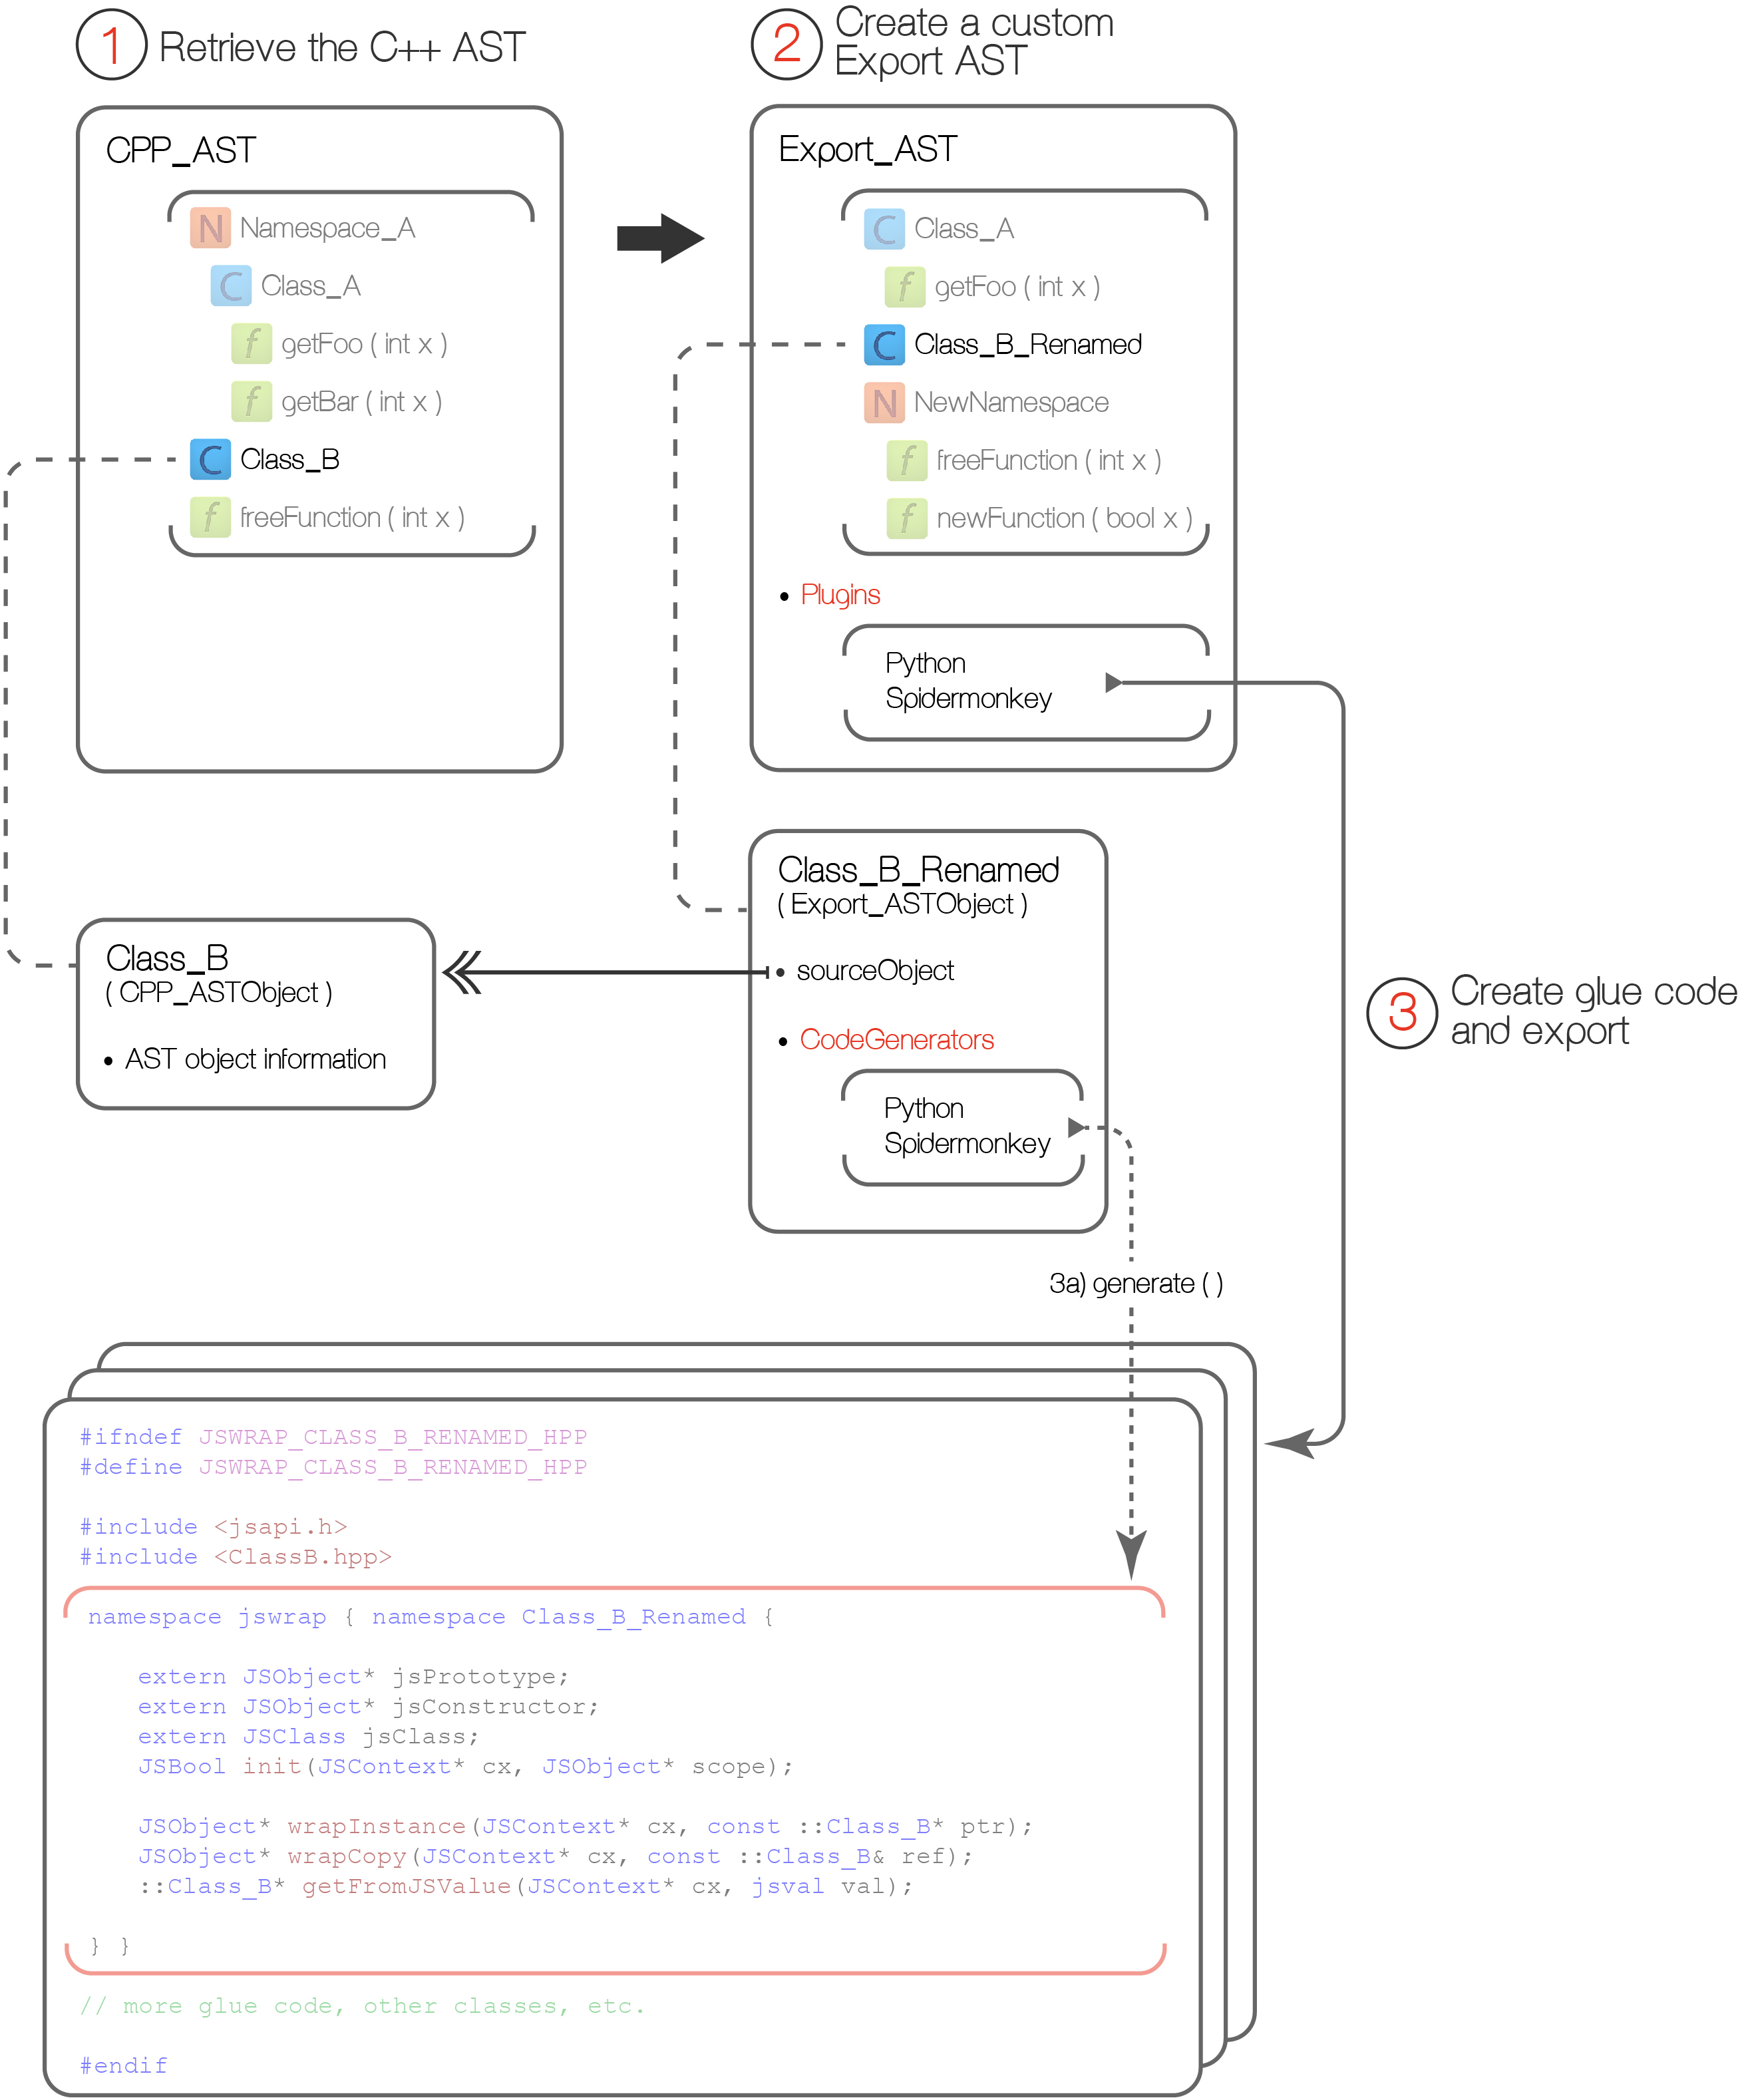
\includegraphics[scale=0.35]{Images/GUIApp_Concept.jpg}
	\caption{Basic concept}
	\label{fig:GUIAppConcept}
\end{figure}

In the first step, the application retrieves the \myProperName{C++} AST of a given source code file using \myProperName{CPPAnalyzer}. The data structures closely (but not completely) resemble the data structures used in \myProperName{CPPAnalyzer}. The information about the tree is hold in an instance of the \myProperName{JavaScript} class \mySCName{CPP\_AST} (equivalent to \mySCName{Clang\_AST}). This object holds a reference to the root tree node. All tree nodes are instances of subclasses of \mySCName{CPP\_ASTObject}.

Based on the elements in the \myProperName{C++} AST, the user will create a custom Export AST. This gives him the opportunity to alter the output of the application by choosing the AST nodes to be exported, rearranging the hierarchy and adding (artificial) nodes that are not in the original \myProperName{C++} AST. This gives the user complete control about how his C++ code can be accessed from script. Similar to \mySCName{CPP\_AST}, \mySCName{Export\_AST} holds a reference to the root tree node of the export tree. All tree nodes are instances of \mySCName{Export\_ASTObject}.

Both \mySCName{CPP\_AST} and \mySCName{Export\_AST} share the same base class \mySCName{AST}. \mySCName{ASTObject} is the base class of \mySCName{CPP\_ASTObject} and \mySCName{Export\_ASTObject}.

The glue code will be generated with the help of special code generator plugins/language plugins. The application can be extended to support glue code generation for arbitrary scripting languages. Based on the list of installed plugins, the user can add multiple plugins to the the existing \mySCName{Export\_AST}. In \myRefFigure{fig:GUIAppConcept} the plugins for \myProperName{Python} and \myProperName{Spidermonkey} have been added, while plugins for \myProperName{LUA} or \myProperName{PHP} may be installed, but are not needed for the user's project.

Every \mySCName{Export\_ASTObject} holds a list of code generators. Code generators are special classes provided by a plugin, which have the objective of generating the glue code for the specific \mySCName{Export\_ASTObject} they are connected to. The information used for the glue code generation is mostly retrieved from the \mySCName{Export\_ASTObject}s \mySCName{sourceObject}, which is usually a reference to a \mySCName{CPP\_ASTObject}. In \myRefFigure{fig:GUIAppConcept} \mySCName{Class\_B\_Renamed} uses the \myProperName{C++} class \mySCName{Class\_B} as its \mySCName{sourceObject}. Code generators also have a set of options that can be altered to influence the glue code generation.
Every plugin comes with a set of code generators that handle the different kinds of \mySCName{CPP\_ASTObject}s. Thus a plugin provides different code generators for handling functions, classes, and so on. 

When performing the final export of a plugin, it traverses all the \mySCName{Export\_ASTObject}s in the tree, uses the associated code generators to produce glue code pieces that are then combined and saved in files. These files can be included in \myProperName{C++} projects and used in conjunction with the embedded script interpreter to add script-support for the wrapped classes and functions.

\section{Architecture}

The application mainly contains three different types of files:

\begin{itemize}\addtolength{\itemsep}{-0.5\baselineskip}
\item \myProperName{XUL} files contain markup for the layout of the GUI
\item \myProperName{CSS} files provide design information for the GUI markup
\item \myProperName{JavaScript} files provide the programming logic for the GUI and the internal parts of the application
\end{itemize}

Most of the \myProperName{JavaScript} logic is placed in modules that are shared across multiple windows. As the \myProperName{JavaScript} language itself does not support module files (as, for example \myProperName{Python} does), \myProperName{Mozilla} integrated module support in \myProperName{XULRunner} with \myProperName{JavaScript code modules}\footnote{\url{https://developer.mozilla.org/en/JavaScript_code_modules/}}. These modules can be imported from any \myProperName{JavaScript} file using a special import command.

The \mySCName{Bound} module is the main module of the application and can be imported to have access to the whole application. It stores information about the current project and holds a reference to the main window in case access to the GUI elements is needed.

The \mySCName{CPPAnalyzer} module provides access to the \myProperName{CPPAnalyzer} library and as such is used for parsing \myProperName{C++} files and retrieving the AST information.

For easier maintenance, application logic and GUI logic is separated. All modules that provide logic for the user interface and specific GUI elements are in a subfolder called \mySCName{UI}. None of these modules is referenced from code outside of this folder, except by \myProperName{XUL} files and the \mySCName{Bound} module. This will make it easier to develop a command-line version of \myProperName{Bound} at some point in the future.

\subsection{Meta data}

A meta data system has been developed to equip \myProperName{JavaScript} objects (and ''classes'') with additional information that can be used for dynamic GUI element creation and serialization/deserialization.

It can be used after importing the \mySCName{MetaData} module.

\SingleSpacing
\begin{lstlisting}[language=JavaScript, caption=Adding meta data to \myProperName{JavaScript} objects]
Components.utils.import("chrome://bound/content/modules/MetaData.jsm")

function SomeClass()
{
	this._notImportant = "This member is neither viewable nor savable";
	this.editMe = "This member will be shown and editable in the GUI";
	this.saveMe = "This member will be saved upon serialization";
	this.showAndSaveMe = "This member is viewable (but readonly)
	                      and savable";
}

MetaData.initMetaDataOn(SomeClass.prototype)
   .addPropertyData("editMe",        { view: {}})
   .addPropertyData("saveMe",        { view: {}, load_save: {}})
   .addPropertyData("showAndSaveMe", { view: {readOnly: true}, 
                                       load_save: {}})
\end{lstlisting}
\OnehalfSpacing

The call to \mySCName{initMetaDataOn} will create a non-enumerable property called \mySCName{\_metaData} on the given object. \mySCName{addPropertyData} adds information about the property with the given name. What kind of data is provided depends on how the object shall be used in the future.
\\The \mySCName{ObjectExplorer} (see \myRefSection{sec:ObjectExplorer}), for example, will check every enumerable property to see if a) it contains meta data and b) if that meta data has the \mySCName{view} member. If so, the checked property (e.g. \mySCName{editMe}) will be visible, when the object is inspected and depending on the type of the property (which can also be forced in the \mySCName{view} object) a GUI element will be created dynamically.
\\The \mySCName{LoadSaveFromMetaData} module  (used in \myRefSection{sec:Project}), on the other hand, can be used to serialize and deserialize an object with \myProperName{JSON}. It checks the meta data for the existence of the \mySCName{load\_save} member. If it exists, the checked property (e.g. \mySCName{saveMe}) can be saved/loaded. The saving or loading process can be customized by providing \mySCName{save} and \mySCName{load} functions with the \mySCName{load\_save} object. If such functions are not provided, the property will be saved according to its type.

The meta data is usually not used in its raw state. As an instance of a class that inherits from another class can contain multiple meta data objects (for the base class, for the subclass and even for the instance itself), the meta data will usually be aggregated before using it. \mySCName{MetaDataAggregate} performs this task by traversing the prototype chain and collecting all existing meta data objects. If multiple meta data objects contain data about the same property, the data of the subclass shadows the data of the base class for that property.

The meta data system is a core component of the application and plays a grand role in the maintainability of the source code as well as the customizability of the generated output and the application itself.

\section{The \myProperName{C++} AST}

The \myProperName{C++} is retrieved by calling the \mySCName{parse\_header} function of the \myProperName{CPPAnalyzer} shared library (see \myRefSection{sec:CallingCPPAnalyzer}).

As \myProperName{CPPAnalyzer} exposes a \myProperName{C} interface, it can be used from \myProperName{JavaScript} with the help of \myProperName{js-ctypes}. As explained in \myRefSection{sec:DynamicFFI}, glue code needed to be written in \myProperName{JavaScript} to wrap the functionality of the library. The \mySCName{CPPAnalyzer} module contains the according code and can be imported to use the \myProperName{CPPAnalyzer} library.

\mySCName{parse\_header} returns the stringified JSON representation of the \myProperName{C++} AST, as shown in \myRefSection{sec:ExportJSON}. The string is deserialized into a \myProperName{JavaScript} object using \myProperName{JavaScript}'s \mySCName{JSON.parse} function.

In the next step an instance of \mySCName{CPP\_AST} including the AST nodes (\mySCName{CPP\_ASTobject}s) needs to be created from the result object. The AST nodes from \myProperName{CPPAnalyzer} shown in \myRefFigure{fig:ASTObjectUML}: \textbf{\mySCName{ASTObject} classes and \mySCName{ASTType}} have equivalents in \myProperName{JavaScript}, which mostly have the same properties. The \myProperName{JavaScript} class \mySCName{CPP\_ASTObject\_Namespace}, for example, is the equivalent to the \myProperName{C++} class \mySCName{ASTObject\_Namespace}.\\
The result object is traversed and \mySCName{CPP\_ASTObject}s and \mySCName{CPP\_ASTType}s created from the according objects. As the AST nodes and types cross-reference each other, this happens in two steps. This is necessary, because an object referenced may not have been created yet in case it is defined later in the tree.\\
First, instances of the according classes are created, but only with information about the name, id and parent of the AST object. Thus the final tree is already formed, though lacking specific information about its members. Types are created in a similar way. For both, the newly created objects are kept track of with a map that associates ids and AST nodes.\\
In the second step, the created objects are updated and missing information for all nodes and types is retrieved. If a cross-reference is found, the according AST node or type is looked up using the id-maps.

\section{The Export AST}

\section{Code generation}

This section will explain the basic concept behind code generation plugins, especially for language bindings. Adding code generation support for a scripting language is exemplified with the code generation plugin written for \myProperName{Mozilla Spidermonkey}.

As explained in \myRefSection{sec:BasicConcept}, the code generation is not based on the \myProperName{C++} AST itself, but on an export AST, whose \mySCName{Export\_ASTObject}s reference the \mySCName{CPP\_ASTObject}s as their \mySCName{sourceObject}. The export AST only includes the nodes the user wants to export. The nodes can be rearranged, renamed and ''artificial'' nodes can be added. 

To create glue code for a specific scripting language, the user needs to add an instance of the according language plugin to the export AST. The language plugin only controls the code generation and exports the final files. The creation of the glue code itself happens with the help of the entity code generators. If the user wants to export a specific \myProperName{C++} entity to \myProperName{Spidermonkey}, for example the function \mySCName{foo}, an instance of the \myProperName{Spidermonkey} function code generator needs to be added to the according \mySCName{Export\_ASTObject}. The entity code generators come with the according language plugin. All in all this means that the user can create \textbf{one} export AST for exporting glue code for \textbf{multiple} languages. If an \mySCName{Export\_ASTObject} does not have an entity code generator for a specific target language, this object is simply not exported for that language.

Every language plugin inherits from the class \mySCName{LanguageBindingCodeGenPlugin}, which itself inherits from \mySCName{BaseCodeGenPlugin}. As the name suggests \mySCName{BaseCodeGenPlugin} defines the basic functionality for all kinds of code generation plugins (e.g. type library or documentation generators), whereas \mySCName{LanguageBindingCodeGenPlugin} adds functionality related to language binding. The entity code generators themselves have a similar hierarchy, inheriting from \mySCName{LanguageBindingEntityCodeGen}, which inherits from \mySCName{BaseEntityCodeGen}.

\mySCName{BaseCodeGenPlugin} provides dummy implementations for loading and saving the plugin. Every plugin also has to provide a property named \mySCName{context}, which declares the purpose of the plugin. The \mySCName{context} of the \myProperName{Spidermonkey} plugin is ''CPP\_Spidermonkey'', as it binds C++ and Spidermonkey. The \mySCName{context} is the entry under which plugins are stored in the \mySCName{Export\_AST} (and entity code generators in the \mySCName{Export\_ASTObject}).
\\Every instance of \mySCName{BaseEntityCodeGen} and its subclasses stores a reference to the plugin it was created from and to the \mySCName{Export\_ASTObject} for which it generates code. Besides dummy implementations for loading and saving, the \mySCName{BaseEntityCodeGen} also contains dummy implementations for \mySCName{prepareAndDiagnose} and \mySCName{generate}. These are the two main functions used in the generation process and will be explained in more detail later.

\subsection{Templates}

There are different ways of creating glue code for a target language. The generated glue code may make use of \myProperName{C++} features like namespaces, exceptions or templates. There a valid reasons, why an end-user might not want to or cannot use these features. If a scripting language provides a \myProperName{C}-API, it should be possible to create glue code in plain \myProperName{C}. Either way, the language plugin should not dictate the glue code style preferred by its developer.

For this reason, entity code generators make use of templates (not to confuse with \myProperName{C++} templates). A template is basically a string of ''incomplete'' source code. It is ''incomplete'' in the sense that it contains place holders that will be filled with proper code when processing the template with the template engine. The template engine used in this project is \myProperName{jSmart}\todo{ref}, a \myProperName{JavaScript} port of the \myProperName{PHP} template engine \myProperName{Smarty}\todo{ref}.

\newpage
\SingleSpacing
\begin{lstlisting}[language=JavaScript, caption=Template for converting a \mySCName{bool} to \myProperName{JavaScript} in \myProperName{Spidermonkey}, label=lst:TemplateBool]
// declaring a template for converting a C++ bool to JS
var code = "jsval {$jsvalName} = BOOLEAN_TO_JSVAL({$inputVar});";

// creating the template
var template = new jSmart(code);

// processing the template
var result = template.fetch({jsvalName: "jsBool", 
                             inputVar:  "cppBool"});
                             
// result --> "jsval jsBool = BOOLEAN_TO_JSVAL(cppBool);"
\end{lstlisting}
\OnehalfSpacing

As can be seen in \myRefListing{lst:TemplateBool}, the template code contains the placeholders \mySCName{\{\$jsvalName\}} and \mySCName{\{\$inputVar\}}. After creating the \myProperName{jSmart} template by calling the \mySCName{jSmart} constructor, the \mySCName{fetch} function can be used to process the template. The function requires an argument that contains the values to be inserted for the placeholders (''jsBool'' and ''cppBool'').

Thus, the entity code generator's main task is to collect all the information needed, checking it for validity and passing it on to the template(s) for creating the final glue code. The code generator should thus be agnostic to different styles of glue code.

Template manager: paths and shadowing\todo{here}


Using templates for glue code generation categorizes the developers/users into four groups: besides the \myProperName{Bound} main developers and language plugin developers, there are language plugin template developers that create complete sets of templates (e.g. one set that creates glue code in plain \myProperName{C}, another that uses \myProperName{C++} features, etc.). End-users will decide for a set and only shadow single templates for customizing the export of specific kinds of entities or change a code generator to use a different template for its connected \mySCName{Export\_ASTObject} only.



code generators, templates, 
    TypeSystem
        Shadowing of templates
    Templates
        templating using jSmart
        templates in JSON for additional data
        problem with escaping newline and tab
        includes
        custom functions (die auch auf alles zugreifen können, z.b. log) -> fungieren genauso als return-values!

type printer
\subsection{The Spidermonkey code generator}

type libraries

\section{The project}
\label{sec:Project}

saving and loading, reparsing, metadata, etc., versioning

\section{GUI widgets}

\subsection{ObjectExplorer}
\label{sec:ObjectExplorer}

\subsection{DOMTree}

\section{GUI overview}

\section{Known Problems}

from which file was a symbol included: need include file hierarchy


